% IMS
% Projekt
% Juraj Holub
% xholub40@stud.fit.vutbr.cz

\documentclass[a4paper, 11pt]{article}
\usepackage[utf8]{inputenc}
\usepackage[czech]{babel}
\usepackage[IL2]{fontenc}
\usepackage{times}
\usepackage[left=1.5cm,top=2.5cm,text={18cm,25cm}]{geometry}
\usepackage[unicode]{hyperref}
\usepackage{amsmath, amsthm, amsfonts, amssymb}
\usepackage{dsfont}
\setlength{\parindent}{1em}
\usepackage{hyperref}
\usepackage{graphicx}
\usepackage{float}
\usepackage{wrapfig}
\usepackage{listings}
\usepackage{url}
\usepackage{cite}

%\date{}

\lstset{
	basicstyle=\small\ttfamily,
}

\begin{document}
\begin{titlepage}
	\begin{center}
		\Huge
		\textsc{Fakulta informačních technologií \\
			Vysoké učení technické v~Brně} \\
		\vspace{\stretch{0.382}}
		{\LARGE
			IMS - Modelování a simulace \\ 
			\medskip 
			\Large{
				Ohrev užitkovej vody v rodinnom dome solárnym systémom.
			}
			\vspace{\stretch{0.618}}}
		\setlength{\parindent}{0.3em}\\
		{\Large 2019} \\
		{\Large Juraj Holub (xholub40)}\\
		{\Large Matej Parobek (xparob00)}
	\end{center}
\end{titlepage}

\tableofcontents
\newpage

\section{Úvod}
Stavebníctvo má v dnešnej dobe veľký dopad na životné prostredie. Spôsob získavania tepelnej energie pre ohrev obytných objektov pomocou alternatívnych zdrojov produkuje nezanedbateľne menšie množstvo CO$_2$ spalín. Táto práca analyzuje systém na ohrev užitkovej vody pre konkrétny rodinný dom. Simulačný model zhodnocuje dopad získavania tepelnej energie zo solárnych panelov na životné prostredie a návratnosť tejto investície v čase. 

\subsection{Zdroje infromácií a autori práce}
Konkrétna špecifikácia a hodnoty požiadaviek na tepelnú energiu v dome vychádzajú z nasledujúcej práce \cite{bc_solar_system}. Prácu vytvoril vedecký pracovník Energetického ústavu Fakulty strojního inženýrství VUT v Brne Ing. Ján Tuhovčák, Ph.D. ako záverečnú prácu a úspešne ju obhájil s klasifikáciou A. Cena na vybudovanie systému vychádza taktiež s tejto práce. Cena fosilných palív je získaná z aktuálneho cenníku čierneho uhlia pre November 2019 \cite{ceny_paliva}. Simulačný model vytvorili Juraj Holub A Matej Parobek na základe týchto informácií. 

\subsection{Validácia navrhovaného modelu}
Práca s ktorej model vychádza poskytuje ročné vyhodnotenie z hľadiska energetických nárokov objektu. Výsledky modelovej simulácie pre rovnaké časové obdobie sa zhodovali s týmito podkladmi. Z tohto hľadiska bol model vyhodnotený ako validný.


\section{Rozbor navrhovaného systému a použitých technológií}

V rodinnom dome je v prevádzke systém na ohrem vody pomocu zemného plynu s bežným kotlom. Aktuálna sadzba za plyn potrebný na vyprodukovanie 1 kWh je 4,49 CZK. Vyprodukovaná energia pomocou solárnych panelov je zadarmo ale počiatočná investícia na vybudovanie a nákup solárneho systému o ploche 6m$2$ je 82 000 CZK. V rodinnom dome sa spotreba tepla na ohrev vody pohybuje okolo 309 kWh za mesiac (nezávislo od ročného obdobia). Naopak produkcia tepelnej energie pomocou solárnych panelov je závislá na ročnom období. Pre daný solárny panel a rodinný dom miestom v Brne je vzhľadom na počet dní v mesiaci, strednú teplotu vzduchu, pomernú dĺžku slnečného svitu, sklon kolektorov (30$^{\circ}$) a ich orientáciu (juh), produkcia tepla pre jednotlivé mesiace zobrazená v tabuľke \ref{tab:mesacna_produkcia_solar}.

\begin{table}[h]
	\centering
	\begin{tabular}{|c|c|c|}
		\hline
		\textbf{Mesiac} & \textbf{\begin{tabular}[c]{@{}c@{}}Vyprodukované teplo\\ {[}kWh{]}\end{tabular}} & \textbf{\begin{tabular}[c]{@{}l@{}}Počet dní\\ v mesiaci\end{tabular}} \\ \hline
		I. & 37,232 & 31 \\ \hline
		II. & 112,367 & 28 \\ \hline
		III. & 269,929 & 31 \\ \hline
		IV. & 370,764 & 30 \\ \hline
		V. & 617,854 & 31 \\ \hline
		VI. & 717,653 & 30 \\ \hline
		VII. & 768,901 & 31 \\ \hline
		VIII. & 601,239 & 31 \\ \hline
		IX. & 418,186 & 30 \\ \hline
		X. & 191,496 & 31 \\ \hline
		XI. & 58,362 & 30 \\ \hline
		XII. & 16,692 & 31 \\ \hline
	\end{tabular}
	\caption{Vyprodukované teplo pomocou solárnych panelov pre jednotlivé mesiace.}
	\label{tab:mesacna_produkcia_solar}
\end{table}

Ak solárna energia v danom mesiaci nepostačuje na pokrytie spotrebovaného tepla tak sa požadovaná energia získava sekundárnym zdrojom, ktorým je plynový kotol. Na druhej strane, prebitky solárnej energie sa v navrhovanom systéme vôbec nevyužívajú. Navrhovaný solárny systém neprodukuje žiadne spaliny CO$_2$. Naproti tomu, spaľovanie plynu produkuje 202g CO$_2$ spalín \footnote{Zdroj \href{https://www.oplyne.info/ecology/porovnanie-produkcie-znecistujucich-latok-so2-tzl-nox-co-a-sklenikoveho-plynu-co2-vyprodukovanych-spalinami-v-rodinnom-dome-vykurovanie-drevom-ciernym-hnedym-uhlim-a-zemnym-plynom/}{https://www.oplyne.info/ecology/porovnanie-produkcie-znecistujucich-latok...}}  na 1 kWh vyprodukovaného tepla. Podľa referenčnej práce sú emisie spojené s vybudovaním solárneho systému porovnateľné s emisiami na vybudovanie pôvodného systému. S tohto dôvodu emisie spojené s vybudovaním systému táto práca neuvažuje. 

\subsection{Postup požitý pre vytvorenie modelu}

Zo získaných vstupných informácií bol vytvorneý abstraktný model (IMS\cite{ims_slides} slide 9.) vo forme Petriho siete (IMS\cite{ims_slides} slide 123.). K nemu bol vytvorený ekvivalentný simulačný model(IMS\cite{ims_slides} slide 44.) v programovacom jazyku C++ za použitia knihovny \textbf{SIMLIB}\footnote{Project SIMLIB: \href{http://www.fit.vutbr.cz/~peringer/SIMLIB/.cs}{http://www.fit.vutbr.cz/~peringer/SIMLIB/.cs}} . Knihovna bola zvolená s ohľadom na zložitoť modelu. Použitie robustnejšej knihovny by vzhľadom na náročnosť abstraktného modelu bolo neprimerané. Táto knihovna poskytuje základné prostriedky pre diskrétne modelovanie (IMS\cite{ims_slides} slide 44.) ako sú procesy (IMS\cite{ims_slides} slide 121.) alebo obslužné linky(IMS\cite{ims_slides} slide 138.) a to pomocou prostriedkov Objektovo Orientovaného Programovania (OOP).

\subsection{Povod použitých technológií}
Na vytvorenie Petriho sieťe som využil postupy preberané na predmete IMS\cite{ims_slides} v kapitole \textit{Diskrétní simulace}. Simulačný model som implementoval v jazyku C++ za použitia OOP abstrakcie a funkcionality zo štandardnej knihovny pre štandard z roku 2014. Program prekladám pomocou GNU C++ prekladača \texttt{g++} \footnote{GNU project \href{https://gcc.gnu.org/}{https://gcc.gnu.org/}}. Knihovnu SIMLIB  som využil pod licenciou GNU LGLP \footnote{GNU Lesser General Public License \href{https://www.gnu.org/licenses/lgpl-3.0.html}{https://www.gnu.org/licenses/lgpl-3.0.html}} . 

\section{Konceptuálny model}
Na základe rozboru navrhovaného systému bol vytvorený konceptuálny model (IMS\cite{ims_slides} slide 48.) popísaný v tejto kapitole.  Najmenšia časová jednotka v modeli je jeden deň. Takáto jednotka bola zvolená preto, že hodnoty v systéme máme dostupné vždy pre časové obdobie jeden mesiac a zároveň pre zhodnotenie výstupov musí model simulovať čas minimálne v rádoch rokov. Pre vyhodnotenie modelu budeme pracovať v jednotkách rokov lebo na základe rozboru\footnote{viď. strana 41 \cite{bc_solar_system}} je návratnosť systému približne v období 35 rokov a menšie časové obdobie ako roky by teda neprinieslo hodnotné informácie. 

Najmenšou energetickou jednotkou, ktorú model umožnuje reprezentovať je 1 kWh/deň a to z dôvodov primerane výpočetnej náročnosti vzhľadom na presnosť výpočtu. Mesačné pohyby energie v systéme sú v rádoch stoviek kWh. Cena a emisie pre menšie jednotky tepelnej energie sú zanedbateľne malé. Napríklad pre mesačne vyprodukovaných 500.4 kWh tepla vznikne 500 procesov. Ak by sme chceli reprezentovať energiu o ešte o jeden rád presnejšie tak by pre 500.4 kWh vzniklo 5004 procesov. Výpočetná náročnosť by teda vzrástla 10-násobne ale výpočet by bol presnejší len o 0.4 kWh čo znamená, že výpočet sa spresní približne o 2\%.


\subsection{Petriho sieť} \label{petri_net_section}
Konceptuálny model reprezentovaný pomocou Petriho siete je priložený na obrázku \ref{obr_petri_net}. Linka \textit{Nový mesiac} je uvoľnená a následne obsadená vždy na začiatku nového mesiaca. Na začiatku nového mesiaca sa vygeneruje \textit{n} procesov \textit{Zdroj solárnej energie}, kde \textit{n} je rovné množstvu kWh tepla vyprodukovaného v daný mesiac solárnym panelom. Táto energia sa rozloží na celý mesiac pomocou časovaného prechodu s rovnomerným rozložením (IMS\cite{ims_slides} slide 89.) na intervale pokrývajúcom celý mesiac v jednotkách dňov. Následne každý proces reprezentujúci energiu prioritne prejde do stavu \textit{Spotrebovaná solárna energia} a to práve vtedy ak ešte nebola pokrytá mesačná spotreba energie. Množstvo požadovanej energie určuje linka \textit{Spotreba} s kapacitou 309 čo reprezentuje 309 kWh a teda bežnú mesačnú potrebu energie na ohrev vody. Linka sa vždy na konci mesiaca plne uvoľní. Ak je linka v danom mesiaci už prázdna, tak proces prechádza prechodom \textit{Prebytočná solárna energia}. Tento prechod reprezentuje energiu, ktorá nemá byť ako využitá. V prípade, že v danom mesiaci nebolo vyprodukované dostatočné množstvo solárnej energie na pokrytie spotreby, tak na konci mesiaca na linke \textit{Spotreba} ostáva nenulová kapacita. Táto kapacita na konci mesiaca reprezentujú množstvo energie v kWh, ktorá nebola dodaná solárnym systémom a preto musela byť získaná spaľovaním zemného plynu.


\begin{figure}[h] 
	\centering
	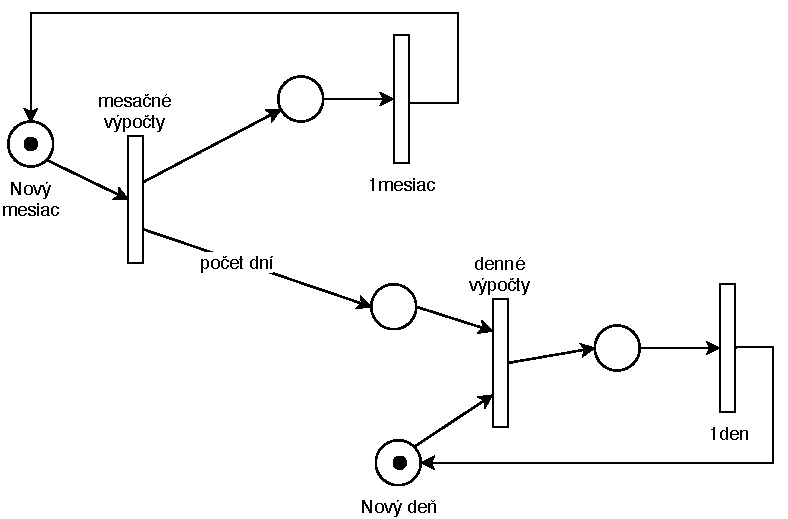
\includegraphics[width=.8\paperwidth]{petri_net.pdf}
	\caption{Navrhnutý konceptuálny model vo forme Petriho siete.}
	\label{obr1}
\end{figure} \label{obr_petri_net}

\section{Architektúra programu}
Priebeh simulácie je veľmi závislý od simulačného času a to špecificky od mesiaca, ktorý je aktuálne simulovaný. Architektúra programu preto implementuje špeciálnu datovú štruktúru ktorej stav uchováva informácie o aktuálnom mesiaci v simulačnom čase. Tok jednej jednotky solárnej energie v priebehu mesiaca je simulovaný jedným procesom. Každý takýto proces vznikne a zanikne v rámci jedného mesiaca. Množstvo aktuálne vygenerovaných procesov opäť závisí od aktuálneho mesiaca. Každý proces pridáva v priebehu simulácie datá do datovej štruktúri, ktorá zaznamenáva štatistické informácie o priebehu simulácie. Proces tieto datá generuje na základe stavu v akom sa aktuálne nachádza. Po uplinutí simulačného času po ktorý mala simulácia bežať je zo získaných štatistík dopočítané potrebné množstvo energie vyprodukovanej spaľovaním zemného plynu, ceny za vykurovanie a vyprodukované emisie.

\subsection{Ročný cyklus}
Ako popisuje sekcia \ref{petri_net_section}, linka \textit{Nový mesiac} je dostupná vždy na začiatku nového kalendárneho mesiaca. Toto chovanie zabezpečuje proces, ktorý linku obsadí, uspí sa na mesiac a linka je na konci mesiaca uvoľnená iným procesom popísaným v sekcii \ref{solar_energy_proces}. Avšak jednotlivé mesiace v roku sa líšia počtom dní. Preto je v rámci celého programu dostupná datová štruktúra, ktorá uchováva aktuálne prebiehajúci mesiac roku, pričom na začiatku je iniciovaná prvým mesiacom každého kalendárneho roku. Pri uvoľnení linky \textit{Nový mesiac} je vždy nastavený ďalší kalendárny mesiac v roku. Toto chovanie sa cyklicky opakuje po uplinutí roku. Táto štruktúra obsahuje pre každý mesiac príslušný počet dní a taktiež množstvo vyprodukovanej solárnej energie v danom mesiaci. Proces mesiaca sa teda vždy uspí na počet dní príslušný aktuálnemu mesiacu a zároveň vygeneruje príslušné množstvo procesov solárnej energie.

\subsection{Solárna energia}\label{solar_energy_proces}
Na 1 kWh vyprodukovanej solárnej energie v aktuálnom mesiaci, vznikne práve jeden proces. Proces sa po svojom vzniku uspí a to na dobu vygenerovanú generátorom pseudonáhodných čísel (IMS\cite{ims_slides} slide 167.) s rovnomerným rozložením \textit{R(0, b-1)}, kde \textit{b} je počet dní v aktuálnom mesiaci. Takto sa spotreba energie rovnomerne rozloží na celý mesiac. Keď je proces aktívny, pokúsi sa obsadiť jedno miesto v linke \textit{Mesačná spotreba}. Linka má kapacitu rovnú celkovej mesačnej spotrebe energie na ohrev vody. Každý proces sa na konci svojho behu pozrie či nie je posledným bežiacim procesom v danom mesiaci. Tieto informácie mu poskytne štatistická datová štruktúra. Ak je posledný, tak uvoľní celú obsadenú kapacitu linky \textit{Mesačná spotreba} a taktiež uvoľní linku \textit{Nový mesiac} čím umožnuje začiatok nového mesiaca.

\subsection{Používanie programu}
Simuláčný čas programu vždy začína v čase 0 a jeho dĺžku môže uživateľ nastaviť v rokoch. ďalej môže uživateľ nastaviť množstvo spotrebovanej solárnej energie za mesiac a to v jednotkách kWh. Program sa dá preložiť spustením priloženého \texttt{Makefile} a následne spustiť:\\
\texttt{./ims-project -y 30 -e 309} \\
Argument \texttt{-y} definuje počet odsimulovaných rokov a argument \texttt{-e} definuje mesačnú spotrebu energie.

\section{Simulačné experimenty}

\newpage
\bibliographystyle{czechiso}
\bibliography{bib}

\end{document}
